\documentclass[a4paper,12pt]{article} 



%Добавляет возможность искать и копировать текст
\usepackage{cmap}

%Убирает пробел между названием таблицы/рисунка и самой таблицей/рисунком
\usepackage{caption}
\captionsetup[table]{skip= -0 cm}
\captionsetup[figure]{skip= -0 cm}

%Выравнивание названия таблиц по левому краю
%\usepackage[nooneline]{caption} 
%Размеры отступов 
\usepackage[left=20mm, top=20mm, right=20mm, bottom=20mm, footskip=10mm]{geometry}

%Рисунки
\usepackage{graphicx}
\usepackage{wrapfig} %обтекание элементов
\graphicspath{{graphs}{figures}}  % папки с картинками

%Русский язык в формулах
\usepackage{mathtext}

%  Русский язык
\usepackage[T2A]{fontenc}			
\usepackage[utf8]{inputenc}			
\usepackage[english,russian]{babel}	

%Готические буквы
\usepackage{amssymb}

% Математика
\usepackage{amsmath,amsfonts,amssymb,amsthm,mathtools} 
\usepackage{wasysym}

%Цветные подписи в таблице
\usepackage[table,xcdraw]{xcolor}

\usepackage{fancyhdr} % Колонтитулы
 	\pagestyle{fancy}
 	\renewcommand{\headrulewidth}{0.3mm}  % Толщина линейки, отчеркивающей верхний колонтитул
 	%\lfoot{Нижний левый}
 	%\rfoot{Нижний правый}
 	\rhead{Белостоцкий Артмемий, Б04-006}
 	%\chead{Верхний в центре}
 	\lhead{Лабораторная работа №4.7.1}
 	% \cfoot{Нижний в центре} % По умолчанию здесь номер страницы
 	
 	
\begin{document} 

%Титульник 
\begin{titlepage}
	\begin{center}
		\large 	МИНИСТЕРСТВО ОБРАЗОВАНИЯ И НАУКИ РОССИЙСКОЙ ФЕДЕРАЦИИ\\
				МОСКОВСКИЙ ФИЗИКО-ТЕХНИЧЕСКИЙ ИНСТИТУТ \\
				(НАЦИОНАЛЬНЫЙ ИССЛЕДОВАТЕЛЬСКИЙ ИНСТИТУТ)\\ 
				ФИЗТЕХ-ШКОЛА ЭЛЕКТРОНИКИ, ФОТОНИКИ \\
				И МОЛЕКУЛЯРНОЙ ФИЗИКИ \\
		
		
		\vspace{4.0 cm}
		Лабораторная работа № 4.7.1 \\ 
		\LARGE \textbf{Двойное лучепреломление}
	\end{center}
	\vspace{3 cm} \large
	
	\begin{flushright}
		выполнил студент 2 курса \\
		{группы Б04-006}\\
		\textbf{Белостоцкий Артемий}\\
		\textbf{Вовк Дмитрий}\\
	\end{flushright}
	
	\vfill

	\begin{center}
	Долгопрудный, 2022 г.
	\end{center}
\end{titlepage}                                                                      


\section*{Цель работы}

Изучение зависимости показателя преломления необыкновенной волны от направления в двоякопреломляющем кристалле; определение главных показателей преломления no -- обыкновенной и ne -- необыкновенной волны в кристалле; наблюдение эффекта полного внутреннего отражения.

\section*{В работе используются}
\begin{itemize}
\item гелий-неоновый лазер
\item вращающийся столик с неподвижным лимбом
\item призма из исландского шпата
\item поляроид
\end{itemize}

\section*{Теоретические сведения}

При падении световой волны на границу изотропной среды в этой среде от границы распространяется одна волна. Если среда анизотропна, то в ней в общем случае возникают две волны, распространяющиеся от границы в разных направлениях и с разными скоростями. Это явление называется \textit{двойным лучепреломлением}

\subsection*{Плоские волны в кристаллах}

Фундаментальные уравнения Максвелла справедливы без всяких изменений и в кристаллических средах. \\
В отсутствие электрических зарядов и токов они имеют вид

\begin{equation}
\operatorname{rot} \vec{H} = \frac{1}{c} \frac{\partial \vec{D}}{\partial t}, \quad  \operatorname{rot} \vec{E} = -\frac{1}{c} \frac{\partial \vec B}{\partial t}
\end{equation}

Если среды прозрачны и однородны, то в них могут распространяться плоские монохроматические волны. Запишем такую волну в комплексном виде:

\[
\vec{E}=\vec{E}_{0} e^{i(\omega t-\vec{k} \vec{r})} ; \quad \vec{B}=\vec{H}=\vec{H}_{0} e^{i(\omega t-\vec{k} \vec{r})} ; \quad \vec{D}=\vec{D}_{0} e^{i(\omega t-\vec{k} \vec{r})}
\]

Заметим, что $\frac{\partial \vec{D}}{\partial t} = i \omega \vec{D}$, т.е. операция дифференцирования сводится к умножению на $i \omega$. Аналогично дифференцирование по координатам x, y, z сводится к умножению на $-ik_x, -ik_y, -ik_z$.

\[
\operatorname{rot} \vec{H}=\left|\begin{array}{ccc}
\vec{e}_{x} & \vec{e}_{y} & \vec{e}_{z} \\
\frac{\partial}{\partial x} & \frac{\partial}{\partial y} & \frac{\partial}{\partial z} \\
H_{x} & H_{y} & H_{z}
\end{array}\right|=-i\left|\begin{array}{ccc}
\vec{e}_{x} & \vec{e}_{y} & \vec{e}_{z} \\
k_{x} & k_{y} & k_{z} \\
H_{x} & H_{y} & H_{z}
\end{array}\right|=-i[\vec{k} \vec{H}]
\]

и аналогично для $\operatorname{rot} \vec{E}$. В результате (1) перейдут в

\[
[\vec{k} \vec{H}]=-\frac{\omega}{c} \vec{D} ; \quad[\vec{k} \vec{E}]=\frac{\omega}{c} \vec{B} .
\]

\newpage

Введем единичный вектор нормали
$\vec{N}$ к фронту волны и скорость распространения фронт а в направлении этой нормали $v$. Тогда $\vec{k}= \frac{\omega}{v} \vec{N}$ и предыдущие соотношения перейдут в

\begin{equation}
\vec{D}=-\frac{c}{v}[\vec{N} \vec{H}] ; \quad \vec{B}=\frac{c}{v}[\vec{N} \vec{E}]
\end{equation}

\begin{wrapfigure}{r}{0.3\linewidth} 
	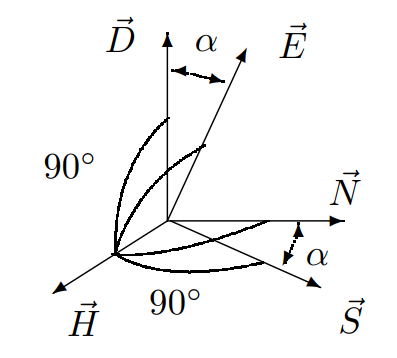
\includegraphics[width=\linewidth]{fig1}
	\caption{Расположение \\ векторов $\vec{D} ,\vec{E}, \vec{N} , \vec{S}$ \\ в анизотропной среде}
\end{wrapfigure}

Отсюда видно, что векторы $\vec{D} , \vec{H} , \vec{N}$ взаимно перпендикулярны. Значит, плоские волны в кристалле поперечны в отношении векторов $\vec{D}$ и $\vec{H}$ . Однако в общем случае они не поперечны в отношении вектора $\vec{E}$

Благодаря тензорной связи между $\vec{D}$ и $\vec{E}$ направления этих векторов в кристаллах, вообще говоря, не совпадают. Плоскость $(\vec{E}, \vec{H})$ обладает тем свойством,что перпендикуляр к ней определяет направление вектора Пойнтинга  \\ $\vec{S} = \frac{c}{4 \pi} \left[ \vec{E}, \vec{H} \right]$


\subsection*{Оптически одноосные кристаллы}

В оптически одноосном кристалле,
каковым является исландский шпат, эллипсоид диэлектрической проницаемости представляет собой эллипсоид вращения. В нем оптическая ось совпадает с осью вращения эллипсоида диэлектрических проницаемостей. Для главных значений диэлектрических проницаемостей приняты обозначения: $\varepsilon_z = \varepsilon_{||}$ и $\varepsilon_x = \varepsilon_y = \varepsilon_{\perp}$.В дальнейшем нам потребуется связь между проекциями векторов $\vec{D}$ и $\vec{E}$ на оптическую ось кристалла ($\vec{D}_{||}$ и $\vec{E}_{||}$) и на плоскость перпендикулярную оси ($\vec{D}_{\perp}$ и $\vec{E}_{\perp}$):

\begin{equation}
\vec{D}_{||} = \varepsilon_{||} \vec{E}_{||}, \qquad \vec{D}_{\perp} = \varepsilon_{\perp} \vec{E}_{\perp}
\end{equation}

\begin{wrapfigure}{r}{0.3\linewidth} 
	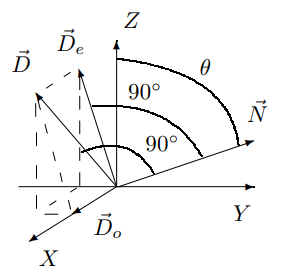
\includegraphics[width=\linewidth]{fig2}
	\caption{Расположение \\ векторов $\vec{D} , \vec{N}$ \\ в анизотропной среде}
\end{wrapfigure}

Волну, распространяющуюся в одноосном кристалле, можно разделить на две линейно поляризованные волны: обыкновенную, вектор электрической индукции $\vec{D}_o$ которой перпендикулярен главному сечению, и необыкновенную, с вектором электрической индукции $\vec{D}_e$, лежащим в главном сечении (рис. 2).Главным сечением кристалла называется плоскость, в которой
лежит оптическая ось кристалла и нормаль к фронту волны

Для обыкновенной волны материальное уравнение имеет такой же вид, как и в изотропной среде, а скорость распространения и ее показатель преломления не зависят от направления распространения:

\[
v_{o}=\frac{c}{\sqrt{\varepsilon_{\perp}}} \quad \text { и } \quad n_{o}=\frac{c}{v_{o}}=\sqrt{\varepsilon_{\perp}} 
\]

Для необыкновенной волны $\varepsilon$ и соответственно  скорость распространения и показатель преломления зависят от угла между оптической осью кристалла и направлением распространения волны.

\begin{equation}
\frac{1}{[n(\theta)]^{2}}=\frac{\sin ^{2} \theta}{n_{e}^{2}}+\frac{\cos ^{2} \theta}{n_{o}^{2}}
\end{equation}

При $n_o - n_e \ll n_0 \ и \ n_e$ (4) можно упростить: $ n(\theta) \approx n_e + (n_o - n_e) \cos^2 \theta$

\newpage

\subsection*{Двойное лучепреломление в призме из исландского шпата.}

Рассмотрим, как по преломлению лучей в кристаллической призме можно определить показатели преломления для обыкновенной и необыкновенной волны. В работе исследуетс я одна из двух призм, составляющих поляризатор (рис. 3).

\begin{figure}[h]
	\begin{center}
	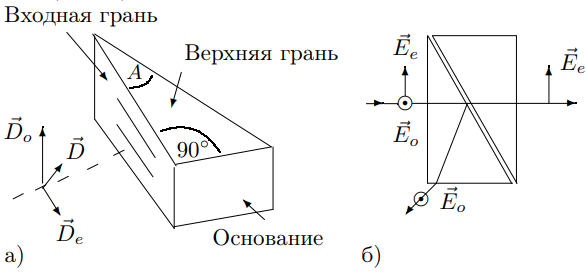
\includegraphics[scale=1]{fig3}
	\caption{а) Исследуемая призма из исландского шпата. Штриховкой указано направление оптической оси кристалла. б) Ход лучей в поляризационной призме}
	\end{center}
\end{figure}

В исследуемой призме ось кристалла лежит в плоскости, параллельной верхней грани призмы, причем она параллельна входной грани призмы (длинному катету). При этом в обыкновенной волне вектор $\vec{D}_o$ перпендикулярен верхней грани призмы, а в необыкновенной волне вектор $\vec{D}_e$ параллелен верхней грани

\begin{wrapfigure}{r}{0.3\linewidth} 
	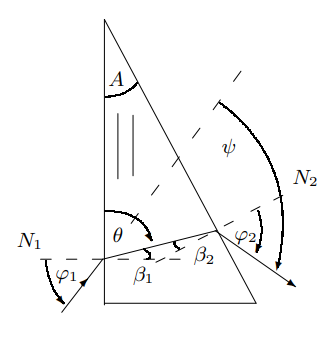
\includegraphics[width=\linewidth]{fig4}
	\caption{Ход лучей в призме}
\end{wrapfigure}

Волну, падающую на входную грань призмы, можно представить в виде суммы двух ортогональных линейно поляризованных волн. Преломление этих двух волн на грани призмы можно рассматривать независимо. Волна, в которой вектор $\vec{D}$ направлен вертикально (перпендикулярно верхней грани и оси кристалла), внутри кристалла будет распространяться как обыкновенная. Для этой волны выполняется закон Снеллиуса, а показатель преломления призмы для нее равен $n_o = \sqrt{\varepsilon_{\perp}}$.Волна, в которой вектор $\vec{D}$ направлен горизонтально, в кристалле будет распространяться как необыкновенная. Для этой волны также будет выполняться закон Снеллиуса, но с тем отличием, что показатель преломления призмы для нее будет зависеть от угла между осью кристалла и волновой нормалью/

Значение показателя преломления и угол, под которым преломилась волна в призме, можно найти, измерив угол падения на входную грань призмы $\varphi_1$ и угол $\varphi_2$ на выходе призмы (рис. 4)

\begin{equation}
n=\frac{1}{\sin A} \sqrt{\sin ^{2} \varphi_{1}+\sin ^{2} \varphi_{2}+2 \sin \varphi_{1} \sin \varphi_{2} \cos A}
\end{equation}

\[
\cos \theta = \frac{\sin \varphi_1}{n}
\]

\newpage

Показатель преломления призмы из изотропного материала
удобно находить по углу наименьшего отклонения луча от первоначального направления. Угол отклонения луча призмой ($\psi$ на рис. 4) минимален для симметричного хода лучей, т.е. когда $\varphi_1 = \varphi_2$. Тогда показатель преломления можно рассчитать по формуле

\begin{equation}
n=\frac{\sin \left(\frac{\psi_{m}+A}{2}\right)}{\sin \left(\frac{A}{2}\right)}
\end{equation}
где $\psi_m$ -- угол наименьшего отклонения

\section*{Экспериментальная установка}

Схема экспериментальной установки изображена на рис. 5. Источником излучения служит Не-Nе лазер ($\lambda$= 0,63 мкм). Излучение лазера поляризовано линейно за счет наличия брюстеровских окошек в кювете лазера. Направление вектора $\vec{E}$ в луче можно изменять с помощью поляроида, установленного на выходе лазера. Исследуемая призма из исландского шпат а закреплена в центре поворотного столик а с неподвижным лимбом для отсчета углов

\begin{figure}[h]
	\begin{center}
	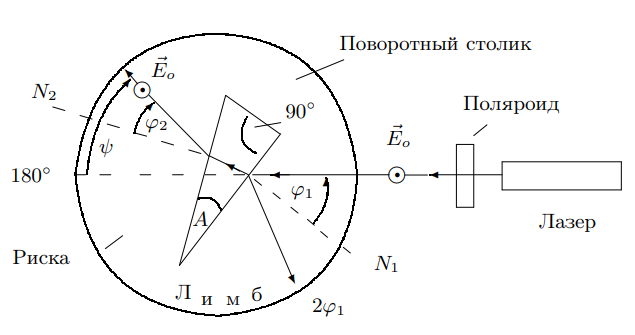
\includegraphics[scale=1]{fig5}
	\caption{Схема экспериментальной установки}
	\end{center}
\end{figure}

\section*{Ход работы}

Определим угол А при вершине призмы: вначале нужно добиться, чтобы луч, отражённый от входной грани (длинного катета), шёл точно назад, заметим положение отсчётной риски на лимбе ($\varphi_1 = 320$\textdegree), а затем повторим эту операцию для второй рабочей грани (гипотенузы) ($\varphi_2 = 180$\textdegree). Тогда угол $А = 180 - (\varphi_1 - \varphi_2) = 38$\textdegree.

Определим разрешенное направление поляризатора, глядя через него на отраженный свет и добиваясь минимума интенсивности.

Получим на лимбе изображение преломленных лучей так, как показано на рис.5. Установим поляризатор в луче перед призмой. Вращая поляризатор, определим какой луч соответствует вертикальной поляризованному свету, а какой горизонтально поляризованному (обыкновенный и необыкновенный лучи).

Вращая столик с призмой, снимем зависимость углов отклонения на выходе из призмы для обыкновенной и необыкновенной волн от угла падения луча на призму. Данные занесем в Таблицу 1.

\begin{table}[h]
\begin{center}
\caption{Зависимость углов отклонения от угла падения}
\begin{tabular}{|c|c|c|c|c|}
\hline
2$\varphi_1$ & $\psi_o$ & $\varphi_{2o}$ & $\psi_e$    & $\varphi_{2e} $\\ \hline
10                         & 36                     & 70                           & 24 						& 58                           \\ \hline
20                         & 32,5                   & 61,5                         & 22                        & 51                           \\ \hline
40                         & 38                     & 57                           & 20,5                      & 39,5                         \\ \hline
60                         & 27                     & 36                           & 20,5                      & 29,5                         \\ \hline
80                         & 27,5                   & 26,5                         & 22                        & 21                           \\ \hline
100                        & 29,5                   & 18,5                         & 25                        & 14                           \\ \hline
120                        & 33                     & 12                           & 28,5                      & 7,5                          \\ \hline
140                        & 38,5                   & 7,5                          & 35                        & 4                            \\ \hline
\end{tabular}
\end{center}
\end{table}

На компьютере в программе SIGMA PLOT по полученным данным построим зависимость $n(\cos^2 \theta)$:

\begin{figure}[h]
	\begin{center}
	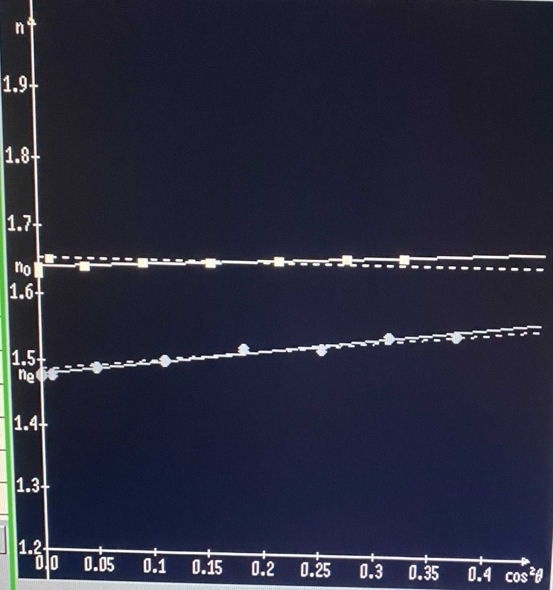
\includegraphics[scale=0.6]{graph1}
	\caption{Зависимость $n(\cos^2 \theta)$ для обыкновенной и необыкновенной волны}
	\end{center}
\end{figure}

Из графика -- $n_e = 1,478 \pm 0.003, n_o = 1,641 \pm 0.005$.

Установим призму так, чтобы были видны оба преломленных луча, затем, уменьшая угол падения, добьемся для каждого из лучей полного внутреннего отражения. Определим соответствующие углы: $\varphi_{1e} = 2$\textdegree, $\varphi_{1o} = -7,5$\textdegree

Тогда по формуле (5) показатели преломления: $n_e = 1,463, n_o = 1,669$

\newpage

\section*{Выводы}

1.В результате работы двумя способами были получены показатели преломления для обыкновенной и необыкновенной волн для исландского щпата.\\
2. Для обыкновенной волны показатели преломления отличаются на 5\%, а для необыкновенной на 1\%


\end{document}